%%
The leading twist tensor structure function $b_1$ quantifies effects not present in 
the case of spin-half hadrons. However the only available targets to study the 
tensor polarization effects on the nucleon substructure are nuclei. 
A measurement of $b_1$ would allow us to take 
a deeper look at the nucleus internal dynamics as $b_1$ should be zero if the 
nucleus is made up of spin-half constistuents at rest, or in a relative $s$-wave. 
Therefore a non-negligible value of $b_1$ can be understood in terms of the deviation 
of a nucleus from a simple bound state of protons and neutrons.
%
\subsubsection{Conventional Nuclear Effects}
The deuteron is the simplest spin-1 many-body nuclear system. In Ref.~\cite{Hoodbhoy:1988am},
the authors evaluate the value of $b_1$ in three different scenarios for the deuteron
constituents and their dynamics:
\begin{enumerate}
 \item[I.] The deuteron is composed of two spin-1/2 non-interacting nucleons at rest. 
In this case, the eight helicity amplitudes characteristic of a spin-1 target are 
expressed in terms of the four helicity amplitudes of each spin-1/2 nucleons, and 
therefore the total number of independent amplitudes is reduced from eight to four. All structure 
functions of the deuteron are then the simple sum of the structure functions of the two 
nucleons, and the tensor structure functions vanish: $b_1 = b_2 
= b_3 = b_4 = 0$. 
 \item[II.] The deuteron is composed of two spin-1/2 nucleons moving non-relativistically 
in a central potential. The target motion modifies the helicity amplitudes. Using
the convolution formalism, it was found that the contribution of these moving nucleons
to $b_1$ is small and is dominated by the lower component of the nucleon's Dirac
wave function.
 \item[III.] The deuteron contains a $D$-state admixture. Because the proton and the neutron
are moving in opposite directions, an additional term due to the $S-D$ interference 
appears in the convolution procedure. This extra contribution to $b_1$ is predicted
to be even smaller than in the previous case.
\end{enumerate}

However, at the quark level, when considering the case of massless relativistic quark, 
$b_1$ exhibits very large negative values peaked at $x=0.5$~\cite{Hoodbhoy:1988am}.
In this calculation, a meson in the $j=1$ state is formed from the coupling of a $P_{3/2}$ 
massless quark with a spin-1/2 spectator.

\begin{figure}[t]
\begin{center}
%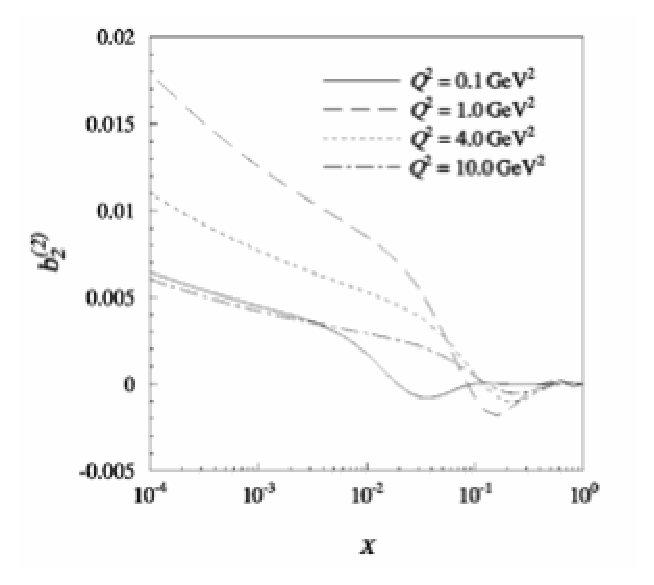
\includegraphics[width=0.40\textwidth]{figs/bora_jaffe_fig3.eps}
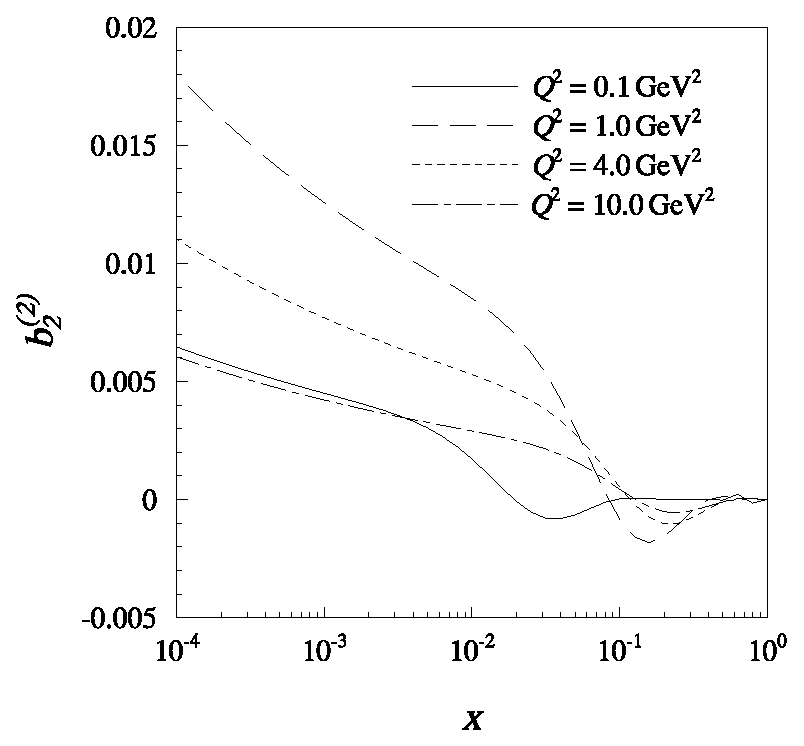
\includegraphics[width=0.3725\textwidth]{figs/bx.eps}
\hspace{0.3cm}
\includegraphics[width=0.45\textwidth]{figs/xb1_mstw_newmiller.eps}
\caption{\label{xb1_pred} Theoretical predictions. {\bf Left plot:} Double-scattering 
contribution to $b_2(x,Q^2)$ as a  function of $x$~\cite{Bora:1997pi}.  Note the strong $Q^2$ dependence at low x.
%($b_2 = b_2^{(1)}+b_2^{(2)}$). 
{\bf Right plot:} HERMES results~\cite{Airapetian:2005cb} compared to calculations 
from S.~Kumano~\cite{Kumano:2010vz} and from the one-pion exchange effects of 
G. Miller~\cite{Miller:1989nc,Miller_tmp}.}
\end{center}
\end{figure}

In 1988, Miller also examined the tensor structure function $b_1$~\cite{Miller:1989nc}.
The basic mechanism is that the virtual photon hits an exchanged pion  which
is responsible for the binding of the deuteron. The calculation depends on the pion 
structure function which carries uncertainty. 
In this early calculation, the convention used by Miller was different from the
one used in the HERMES results and in Ref.~\cite{Kumano:2010vz}. The updated 
calculation~\cite{Miller_tmp} is shown in Fig.~\ref{xb1_pred}. Also the pion structure 
function from~\cite{Sutton:1991ay} was used. The spread of the curve originates from the 
parameter $A_s=(.9 \pm 0.3)$ which governs the strength of the sea in the pion. These 
numbers are all in qualitative agreement with HERMES, given their large error bars.
Another mechanism is expecting to contribute: coherent-double scattering. Miller 
specified that his mechanism is not the same as that, even though the HERMES 
publication~\cite{Airapetian:2005cb} combined them together.

In addition, at $x > 0.2$, a non-negligible value of $b_1^d$ is expected just through
the conventional nuclear effects in the deuteron, Fermi motion and binding~\cite{Khan:1991qk}.

%
\subsubsection{Double-Scattering Effects}
%This leading twist structure function quantifies effects not present
%in the case of spin-half hadrons. It allows a deeper look at the nucleus internal 
%dynamics as $b_1$ should be zero if the nucleus is made up of spin-half constistuents 
%at rest, or in a relative $s$-wave. Therefore a non-negligible value of $b_1$ can be 
%translated into the deviation of a nucleus from a simple bound state of protons and 
%neutrons.
%
Using Vector Meson Dominance (VMD), the authors of Ref.~\cite{Bora:1997pi} isolate the 
double-scattering contribution to $b_1$. The existence time of a vector meson can 
be described by the coherence length $\lambda$: 
\begin{eqnarray}
\lambda = \frac{Q^2}{M x (M_v^2 + Q^2)}
\end{eqnarray}
which is the length over which the vector meson propagates during the time $\Delta t 
= 1/\Delta E$. Therefore, for multiple scattering to occur, a minimum coherence length 
of $\approx$ 1.7 fm (the inter-nucleon separation) is required. At 
$x > 0.3$, the coherence length is only about the size of the nucleon, so multiple 
scattering contributions are anticipated to be negligible. However, for $x \le 0.1$, 
double-scattering should be significant in $b_1$ behaving as $(1-x)^{2\delta}/x^{1+2\delta}$, 
where $\delta$ is determined from the soft pomeron intercept $\alpha_P(t=0) = 1 + \delta$.
Finally the auhors forsee a significant enhancement of $b_1$ at low $x$ ($\le$ 0.01) 
due to the quadrupole deformation of the deuteron.
%\begin{figure}[t]
%\begin{center}
%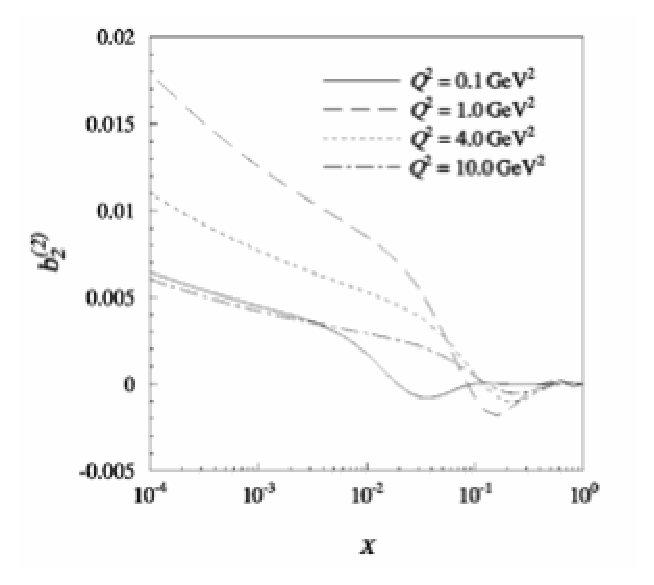
\includegraphics[width=0.5\textwidth]{figs/bora_jaffe_fig3.eps}
%\caption{\label{b2_bora} Double-scattering contribution $b_2^{(2)}(x,Q^2)$ in 
%function of $x$~\cite{Bora:1997pi} (where $2 x b_1 = b_2 = b_2^{(1)}+b_2^{(2)}$).}
%\end{center}
%\end{figure}

\subsubsection{The Close-Kumano Sum Rule}
Following the formalism from the parton model in~\cite{Hoodbhoy:1988am}, Close and 
Kumano ~\cite{Close:1990zw} related the tensor structure function $b_1$ to the electric quadrupole 
form factor of the spin-1 target through a sum rule:
\begin{eqnarray}
\int_0^1 dx~b_1(x)  & = &  - \frac{5}{12 M^2} \lim_{t \rightarrow 0}~t~F_Q(t) 
                           + \frac{1}{9} \Big(\delta Q + \delta \bar{Q}\Big)_s \nonumber \\
                    & = & \frac{1}{9} \Big(\delta Q + \delta \bar{Q}\Big)_s  = 0 \nonumber \\
\label{cksum}
\end{eqnarray}
The sum rule is satisfied in the case of an unpolarized sea. However, the authors emphasize
that in nucleon-only models the integral of $b_1$ is not sensitive to the 
tensor-polarization of the sea, and consequently the sum rule is always true, even when the 
deuteron is in a $D$-state.

Recently, Kumano~\cite{Kumano:2010vz} estimated from an analysis of HERMES data~\cite{Airapetian:2005cb}
that a non-negligible tensor polarization of the sea is necessary to reproduce the trend of
the data. However, this conclusion has to be considered with caution due to the large
$Q^2$ coverage of each HERMES data point (see Fig.~\ref{HERMES_KIN}), and the assumption that 
the sum rule is satisfy for valence quarks.


%



\subsection{Comments from Theorists}
%
During the preparation of this letter, we contacted several theorists 
to gauge interest in a precision measurement of $b_1$.  The response was uniformly positive.  We 
provide some of their feedback for context.
%
%\vspace{0.5cm}
%{\bf S. Kumano (KEK and Tsukuba U.):}
%\vspace{0.5cm}
%{\bf M. Strikman (Penn. State U.) and M. Sargsian (FIU):}
%

\vspace{0.5cm}
``{\it The tensor structure of the deuteron can be investigated in the deep
inelastic region by measuring the structure function $b_1$, which
should shed light on a new aspect of tensor-structure studies in
terms of quark degrees of freedom instead of hadronic ones.
There is a conventional approach for theoretically calculating $b_1$
by quark distribution functions convoluted with nucleon momentum
distributions in the deuteron including the $D$-state admixture.
According to our experience on the nucleon-spin issue, such
a conventional approach for high-energy spin physics would not work.
In particular, it is known that $b_1$ is sensitive to dynamical aspects
of constituents with angular momenta. Measurements of $b_1$ could open
a new field of spin physics because this kind of spin physics has not
been explored anywhere else. Only experimental information came from
the HERMES collaboration; however, their data are not accurate enough
to find $x$ dependence of $b_1$ especially at large $x$. It is
an unique opportunity at JLab to develop this new field of spin physics.}''
\begin{flushright}{\bf S. Kumano (KEK and Tsukuba U.)}\end{flushright}

\vspace{0.5cm}
``{\it I'm glad to hear that $b_1$ is not forgotten in all the excitement about other spin dependent 
effects...
%I don't have much to add to the existing discussion of $b_1$ in the literature. 
%If I remember correctly, 
The hard thing is to distinguish a non-trivial contribution to $b_1$ (eg. 
from 6 quark correlations in the deuteron) from the contribution from the deuteron d-wave.}''
%I 
%also remember a debate about a double scattering contribution.  I wrote a paper on that subject 
%with an Indian visitor to the CTP.  I believe our work was a follow-on to work by Nikolaev and 
%Schafer~\cite{Nikolaev:1996jy}.  I think these papers suggested large contributions to $b_1$ at 
%low x and low $Q^2$.}''
\begin{flushright}{\bf R. Jaffe (MIT)}\end{flushright}

\vspace{0.5cm}
``{\it I am particularly interested in signatures of novel QCD effects in the deuteron. The tensor 
charge could be sensitive to hidden color (non-nucleonic) degrees of freedom at large $x$. It is
also interesting that antishadowing in DIS in nuclei is not universal but depends on the quark 
flavor and spin. One can use counting rules from PQCD to predict the $x \to 1$ dependence of the 
tensor structure function.}''
\begin{flushright}{\bf S. Brodsky (SLAC)}\end{flushright}
 
\vspace{0.5cm}
``{\it I am certainly interested in the experimental development to find the novel
QCD phenomena from the hidden color component of deuteron.}''
\begin{flushright}{\bf Chueng-Ryong Ji (SLAC)}\end{flushright}

